\documentclass[a4paper, 10pt]{scrartcl}


\usepackage{fontspec}
\newcommand{\mainFont}{NotoSerif}
\setmainfont{\mainFont}[
  Path           = ./fonts/\mainFont/static/,
  Extension      = .ttf,
  UprightFont    = *-Regular,
  BoldFont       = *-Bold,
  ItalicFont     = *-Italic,
  BoldItalicFont = *-BoldItalic,
]

\usepackage{xcolor}
\usepackage{tikz}
%\usepackage{lmodern} % Allows arbitrary font scaling without size limits
\usepackage{graphicx}
\usepackage{fontawesome5} % Icons: \faEnvelope, \faPhone, \faGithub, \faLinkedin, \faMapMarker, ...
\usepackage{hyperref} % Clickable mailto:/tel:/http links

\usetikzlibrary{calc} % Required for efficient coordinate calculations

\definecolor{background1}{HTML}{00171f}
\definecolor{background2}{HTML}{00335a}
\definecolor{col3}{HTML}{007da9}
\definecolor{picBorderCol}{HTML}{ffffff}
\definecolor{linkCol}{HTML}{490a83}

% Make links colored instead of the default red/boxed look
\hypersetup{
	colorlinks=true,
	urlcolor=linkCol,
	linkcolor=linkCol,
}

% options for text: \small, \normalsize, \large, \Large, \LARGE, \huge, \Huge

\pagestyle{empty}
\begin{document}

\hyphenpenalty=10000
\exhyphenpenalty=10000

\begin{tikzpicture}[remember picture, overlay, shift={(current page.north west)}]
	% (0,0) is now the top-left corner.




	% --- background ------------------------------------
	\pgfmathsetmacro{\splitpointX}{4}
	\pgfmathsetmacro{\splitpointY}{-5.8}
	\pgfmathsetmacro{\cornerpointUpX}{7.5}
	\pgfmathsetmacro{\cornerpointUpY}{-4.0}

	\pgfmathsetmacro{\cornerpointDownX}{\cornerpointUpX}
	\pgfmathsetmacro{\cornerpointDownY}{-7.8}

	\pgfmathsetmacro{\lastpointX}{4}
	\pgfmathsetmacro{\lastpointY}{-9.0}

	\fill[col3]
        (-1,1) --
        (-1,\lastpointY) --
        % Bézier S-curve connecting the bottom level to the top level
        (\lastpointX,\lastpointY) .. controls (\lastpointX + 2, \lastpointY) and (\cornerpointDownX - 2, \cornerpointDownY) .. (\cornerpointDownX,\cornerpointDownY) --
        (22,\cornerpointDownY) --
        (22,1) --
        cycle;


	\fill[background2]
        (-1,1) --
        (-1,\splitpointY) --
        % Bézier S-curve connecting the bottom level to the top level
        (\splitpointX,\splitpointY) .. controls (\splitpointX + 2, \splitpointY) and (\cornerpointDownX - 2, \cornerpointDownY) .. (\cornerpointDownX,\cornerpointDownY) --
        (22,\cornerpointDownY) --
        (22,1) --
        cycle;

	\fill[background1]
        (-1,1) --
        (-1,\splitpointY) --
        % Bézier S-curve connecting the bottom level to the top level
        (\splitpointX,\splitpointY) .. controls (\splitpointX + 2, \splitpointY) and (\cornerpointUpX - 2, \cornerpointUpY) .. (\cornerpointUpX,\cornerpointUpY) --
        (22,\cornerpointUpY) --
        (22,1) --
        cycle;














	% --- title name ------------------------------------
	\node[anchor=north west, text=white, font=\fontsize{42}{50}\selectfont\bfseries] at (7, -1.0)
	{
		Lucas Furer
	};
	\node[anchor=north west, text=white, font=\fontsize{20}{25}\selectfont] at (7, -2.5)
	{
		Computer Science graduate
	};





	% --- profile pic ------------------------------------
	\pgfmathsetmacro{\picX}{2.9}
	\pgfmathsetmacro{\picY}{-2.9}
	\pgfmathsetmacro{\picS}{2.1}


	\begin{scope}
		\clip (\picX, \picY) circle (\picS cm);
		\node[anchor=north west] at (-3.5 + \picX, 2.5 + \picY)
		{
			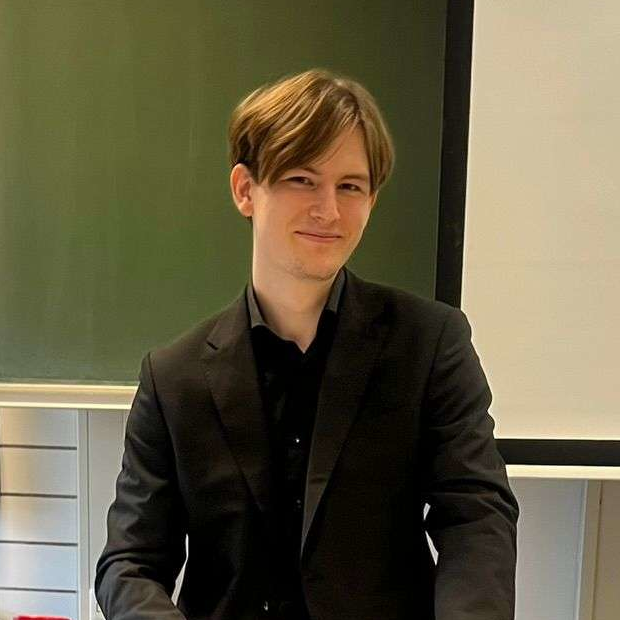
\includegraphics[width=7cm, height=7cm]{figures/new_profile_pic.png}
		};
	\end{scope}
	\draw[picBorderCol, line width=3pt] (\picX, \picY) circle (\picS cm);





	% --- Contact section ------------------------------------
	% \faXXX gives the icon, \href{...}{...} makes it clickable.
	% mailto: opens the default mail client with the address
	% pre-filled; tel: does the same for a phone/dialer app.
	% On both PC and phone PDF readers you can usually also
	% right-click (or long-press) the link to copy it directly.
	\node[anchor=north west, align=left] at (0.5, -5.8)
	{
		\renewcommand{\arraystretch}{1.4}
		\begingroup
		\hypersetup{urlcolor=black}
		\begin{tabular}{@{}l l@{}}
			\faLinkedin   & \href{https://www.linkedin.com/in/lucas-furer-22a38a323/}{lucas-furer} \\
			\faGithub     & \href{https://github.com/LucasFurer}{LucasFurer} \\
			\faEnvelope   & \href{mailto:lucas.furer@gmail.com}{lucas.furer@gmail.com} \\
			\faPhone      & \href{tel:+31652772875}{+31 6 5277 2875} \\
			\faMapMarker  & Delft, NL \\
		\end{tabular}
		\endgroup
	};




	% --- summary ------------------------------------
	\node[anchor=north west, text width=13.2cm,align=left, text=white, font=\large] at (7.0, -4.6)
	{
A detail-oriented and enthusiastic MSc Computer Science graduate with a passion for physics-based simulations, computer graphics and open-source principles. I am an eager learner who enjoys collaborating with others and exploring new technologies. Experienced with C++, Java, GLSL and Python.
	};










	% --- section variables ------------------------------------
	\coordinate (sectStart) at ($(3.9,-9.2)$);


	\pgfmathsetmacro{\horGapSmall}{0.15} % space between text and the line
	\pgfmathsetmacro{\horGapLarge}{16.0} % space between line and dates
	\pgfmathsetmacro{\textWidth}{15.5} % width of the text

	\pgfmathsetmacro{\vertTextGap}{0.05} % spacing between text
	\pgfmathsetmacro{\vertSubGap}{0.1} % spacing between sub headers
	\pgfmathsetmacro{\vertSectGap}{0.3} % spacing between sections






	% --- education ------------------------------------
	\coordinate (eduStart) at ($(sectStart)$);


	\node[anchor=north east, align=left, font=\Large] 
		at ($(eduStart) + (-\horGapSmall,0)$)
	{
		\textbf{Education}
	};


	\node[anchor=north west, align=left, text width=\textWidth cm] (eduEntryA) 
		at ($(eduStart) + (\horGapSmall,0)$)
	{
		\textbf{M.Sc. Computer Science}, \textit{TU Delft}\\
		$\bullet$ \textbf{Thesis:} \href{https://repository.tudelft.nl/record/uuid:67d958d3-0b23-4e1f-b2a1-9c183e590d57}{\textbf{FMM-t-SNE}} Implemented a fast multipole N-body solver and integrated it into t-SNE. Developed in C++ with OpenGL visualization\\
		$\bullet$ \textbf{Grade:} 8.5\\
		$\bullet$ \textbf{Notable courses:} Image Processing, Graphics and Animation, Geometric data Processing\\
	};
	\node[anchor=north east, align=left] 
		at ($(eduEntryA.north west) + (\horGapLarge,0)$)
	{
		\textbf{2023-2026}
	};


	\node[anchor=north west, align=left, text width=\textWidth cm] (eduEntryB)
		at ($(eduEntryA.south west) + (0,-\vertTextGap)$)
	{
		\textbf{B.Sc. Computer Science}, \textit{TU Delft}\\
		$\bullet$ \textbf{Thesis:} \href{https://resolver.tudelft.nl/uuid:80fc65a8-db1c-439c-ad55-46d94739ab02}{\textbf{Soft Peaks}} Studied how the distribution of ray reflections evolve as smoothing is applied to microstructures. Implemented in C++ with results rendered to \texttt{.ppm}\\
		$\bullet$ \textbf{Grade:} 7.5\\
		$\bullet$ \textbf{Minor:} Security, Safety \& Justice\\
		$\bullet$ \textbf{Notable courses:} Linear Algebra, Big Data Processing, Computer Graphics\\
	};
	\node[anchor=north east, align=left] 
		at ($(eduEntryB.north west) + (\horGapLarge,0)$)
	{
		\textbf{2019-2023}
	};


	\coordinate (eduEnd) at ($(eduStart |- eduEntryB.south)$);
	\draw[background2, line width=1pt]
		($(eduStart)$) --
		($(eduEnd)$);

	










	% --- experience ------------------------------------
	\coordinate (expStart) at ($(eduEnd) + (0,-\vertSectGap)$);


	\node[anchor=north east, align=left, font=\Large] (expHeader)
		at ($(expStart) + (-\horGapSmall,0)$)
	{
		\textbf{Experience}
	};
 
 
	\node[anchor=north west, align=left, text width=\textWidth cm] (expEntryA)
		at ($(expHeader.south -| expStart) + (\horGapSmall,0)$)
	{
		\textbf{Feedback Analytics}, \textit{Software Engineer}\\
		$\bullet$ Developed a visualization tool for user-created questionnaires using Angular 13\\ 
		$\bullet$ Lead a five-person team, collaborating closely with the client to gather requirements
	};
	\node[anchor=north east, align=left, font=\normalsize] 
		at ($(expEntryA.north west) + (-2 * \horGapSmall,0)$)
	{
		\textit{Internship}
	};
	\node[anchor=north east, align=left] 
		at ($(expEntryA.north west) + (\horGapLarge,0)$)
	{
		\textbf{2022}
	};


	\node[anchor=north west, align=left, text width=\textWidth cm] (expEntryB)
		at ($(expEntryA.south west) + (0,-\vertSubGap)$)
	{
		\textbf{Blender Addon}, \textit{Author}\\
		$\bullet$ Created a Blender addon that generates terrain using simulated hydraulic erosion\\
		$\bullet$ \textbf{Source Code:} \href{https://github.com/LucasFurer/my_blender_addon}{https://github.com/LucasFurer/my\_blender\_addon}
	};
	\node[anchor=north east, align=left, font=\normalsize] 
		at ($(expEntryB.north west) + (-2 * \horGapSmall,0)$)
	{
		\textit{Projects}
	};
	\node[anchor=north east, align=left] 
		at ($(expEntryB.north west) + (\horGapLarge,0)$)
	{
		\textbf{2026}
	};


	\node[anchor=north west, align=left, text width=\textWidth cm] (expEntryC)
		at ($(expEntryB.south west) + (0,-\vertSubGap)$)
	{
		\textbf{Independent Game Development}, \textit{Software Engineer}\\
		$\bullet$ Organized a four-person team to create a game using Unity and C\# \\
		$\bullet$ Developed procedural terrain generation using Perlin noise and the Marching Cubes\\ algorithm
	};
	\node[anchor=north east, align=left] 
		at ($(expEntryB.north west) + (\horGapLarge,0)$)
	{
		\textbf{2025}
	};


%	\node[anchor=north west, align=left, text width=\textWidth cm] (expEntryC)
%		at ($(expEntryB.south west) + (0,-\vertTextGap)$)
%	{
%		\textbf{Blender plugin}, \textit{CS4540 Geometric Data Processing university course}\\
%		$\bullet$ Developed Blender plugins in python using algorithms such as Constrained Laplace Smoothing, Point-to-Point ICP, Point-to-Plane ICP and KD-tree nearest-neighbor search \\
%		$\bullet$ Conducted experimental performance analysis, comparing convergence speed, registration accuracy and algorithm trade-offs across multiple 3D datasets.
%	};
%	\node[anchor=north east, align=left] 
%		at ($(expEntryC.north west) + (\horGapLarge,0)$)
%	{
%		\textbf{2024}
%	};


	\coordinate (expEnd) at ($(expStart |- expEntryC.south)$);
	\draw[background2, line width=1pt]
		($(expStart)$) --
		($(expEnd)$);
 
 
 
 
 
	% --- skills ------------------------------------
	\coordinate (skiStart) at ($(expEnd) + (0,-\vertSectGap)$);


	\node[anchor=north east, align=left, font=\Large] (skiHeader)
		at ($(skiStart) + (-\horGapSmall,0)$)
	{
		\textbf{Skills}
	};


	\node[anchor=north west, align=left, text width=\textWidth cm] (skiEntryA) 
		at ($(skiHeader.south -| skiStart) + (\horGapSmall,0)$)
	{
		\textbf{C++}\\
		Libraries: Boost, Eigen, Fastor, GLM, OpenGL, GLFW, Vulkan%, FFTW
	};
	\node[anchor=north east, align=left, font=\normalsize] 
		at ($(skiEntryA.north west) + (-2 * \horGapSmall,0)$)
	{
		\textit{Programming}
	};
%	\node[anchor=north east, align=left] 
%		at ($(skiEntryA.north west) + (\horGapLarge,0)$)
%	{
%		\textbf{Advanced}
%	};
 
 
	\node[anchor=north west, align=left, text width=\textWidth cm] (skiEntryB)
		at ($(skiEntryA.south west) + (0,-\vertTextGap)$)
	{
		\textbf{C, Python, C\#, Java, GLSL, CUDA, Unity}\\
		Libraries: Numpy, Matplotlib, Pandas, OpenTSNE, Sklearn
	};
%	\node[anchor=north east, align=left] 
%		at ($(skiEntryB.north west) + (\horGapLarge,0)$)
%	{
%		\textbf{Intermediate}
%	};
 
 
	\node[anchor=north west, align=left, text width=\textWidth cm] (skiEntryC)
		at ($(skiEntryB.south west) + (0,-\vertTextGap)$)
	{
		\textbf{x86-Assembly, HTML, CSS, Javascript, Scala, Rocq, Haskell, SQL, MiniZinc}\\
	};
%	\node[anchor=north east, align=left] 
%		at ($(skiEntryC.north west) + (\horGapLarge,0)$)
%	{
%		\textbf{Basic}
%	};
 
 
	\node[anchor=north west, align=left, text width=\textWidth cm] (skiEntryD)
		at ($(skiEntryC.south west) + (0,-\vertSubGap)$)
	{
		\textbf{CMake, Docker, Linux, Bash, Git, Blender, LaTeX}\\	
	};
	\node[anchor=north east, align=left, font=\normalsize] 
		at ($(skiEntryD.north west) + (-2 * \horGapSmall,0)$)
	{
		\textit{Tools}
	};
 
 
	\node[anchor=north west, align=left, text width=\textWidth cm] (skiEntryE)
		at ($(skiEntryD.south west) + (0,-\vertSubGap)$)
	{
		\textbf{Dutch}, Native\quad \quad \textbf{English}, Fluent\\
	};
	\node[anchor=north east, align=left, font=\normalsize] 
		at ($(skiEntryE.north west) + (-2 * \horGapSmall,0)$)
	{
		\textit{Language}
	};
 
 
	\coordinate (skiEnd) at ($(skiStart |- skiEntryE.south)$);
	\draw[background2, line width=1pt]
		($(skiStart)$) --
		($(skiEnd)$);




 
 
	% --- misc ------------------------------------
	\coordinate (misStart) at ($(skiEnd) + (0,-\vertSectGap)$);


	\node[anchor=north east, align=left, font=\large] 
		at ($(misStart) + (-\horGapSmall,0)$)
	{
		\textbf{Extracurricular}\\
		\textbf{Activities}
	};
 
 
	\node[anchor=north west, align=left, text width=\textWidth cm] (misEntryA) 
		at ($(misStart) + (\horGapSmall,0)$)
	{
		\textbf{D.S.M.G. Krashna Musika}, \textit{Bass singer}\\
		$\bullet$ Performed with a classical music student association in concerts across Europe\\
		$\bullet$ Developed teamwork, discipline and performance skills through rehearsals and live\\ performances
	};
	\node[anchor=north east, align=left]
		at ($(misEntryA.north west) + (\horGapLarge,0)$)
	{
		\textbf{2024-2026}
	};


	\node[anchor=north west, align=left, text width=\textWidth cm] (misEntryB) 
		at ($(misEntryA.south west) + (0,-\vertTextGap)$)
	{
		\textbf{D.S.B.V. Yoroshi}\\
		$\bullet$ Practised judo at a student budosport association\\
	};
	\node[anchor=north east, align=left]
		at ($(misEntryB.north west) + (\horGapLarge,0)$)
	{
		\textbf{2024-2025}
	};



	\coordinate (misEnd) at ($(misStart |- misEntryB.south)$);
	\draw[background2, line width=1pt]
		($(misStart)$) --
		($(misEnd)$);






	% --- hobbies ------------------------------------
	\coordinate (hobStart) at ($(misEnd) + (0,-\vertSectGap)$);



	\node[anchor=north east, align=left, font=\Large] 
		at ($(hobStart) + (-\horGapSmall,0)$)
	{
		\textbf{Interests}
	};


	\node[anchor=north west, align=left, text width=\textWidth cm] (hobEntryA) 
		at ($(hobStart) + (\horGapSmall,0)$)
	{
		Playing piano, creating games/simulations, running, bouldering\\
	};


	\coordinate (hobEnd) at ($(hobStart |- hobEntryA.south)$);
	\draw[background2, line width=1pt]
		($(hobStart)$) --
		($(hobEnd)$);















\end{tikzpicture}

\end{document}
